\chapter{Design Analysis}
An algorithm can be defined as a set of precise (i.e., unambiguous) instructions that specify how to solve a given problem. An algorithm can be implemented in multiple ways leading to varying performance and efficiency of the program, for example, using different data structures, data storage options i.e. if the data should be stored in memory or on file system, implementation language, library functions used etc. A design is a result of such numerous decisions made with the goal to achieve a balance between efficiency and optimization. Very rarely is it possible to find the perfect design which would lead to a program performing with the same efficiency for the entire input space. Hence, while making the decisions it is important to evaluate the advantages and disadvantages of the chosen approach. This chapter is therefore dedicated to analyze the design choices made during the implementation. \\

As discussed in Section \ref{sysMod}, the task submitted by the user to the master node is divided into sub-tasks and distributed among the slave nodes of the cluster. The slave nodes perform the allocated work and report the partial output which is merged at the master node. The Figure \ref{lst:FC} summarizes the process. The \textit{MasterPrintingSoftware} follows the steps denoted in the left branch of the flow chart where as the \textit{SlavePrintingSoftware} follows the steps of denoted in the right branch of the flow chart. The \textit{MasterPrintingSoftware} and \textit{SlavePrintingSoftware} design decisions include:
\begin{enumerate}
\item Format of the sub-tasks allocated to the slaves nodes
\item Distribution of sub-tasks by the master
\item Format of the slave partial output 
\item Merging of the partial output 
\end{enumerate}

\begin{figure}
\centering
\begin{tikzpicture}[node distance=2.75cm] 
\node (start) [startstop] {Start};
\node (dec1) [decision,below of=start ,yshift=-0.75cm]{ Is master node?};
\node (Min1) [io, below left of=dec1 , xshift= -2cm] {Input main configuration file};
\node (Sin1) [io,below right of=dec1 , xshift= 2cm] {Receive sub-tasks from Master};
\node (Mpro1) [process, below of=Min1] {Parse Input, Create sub-tasks, Distribute Sub-tasks};
\node (Mpro2) [process, below of=Mpro1 ,yshift=-0.5cm] {Receive meta-data, compute full slice height, width, offset};
\node (Mpro3) [process, below of=Mpro2 ,yshift=-0.5cm] {Receive partial slices and merge to full slice};
\node (Mdec1) [decision,below of=Mpro3, yshift=-0.5cm]{ Is last slice?};
\node (Spro1) [process, below of=Sin1] {Perform application specific computation and generate chunk-wise slices };
\node (Sdec1) [decision,below of=Spro1, yshift=-0.5cm]{ Is first chunk?};
\node (Spro2) [process, below left of=Sdec1,xshift= -1cm] {Send meta-data to the master};
\node (Spro3) [process, below of=Sdec1,yshift=-1cm ] {Send the partial slice to the master};
\node (Sdec2) [decision,below of=Spro3, yshift=-0.5cm]{ Is last chunk?};
\node (Mend) [startstop,below of= Mdec1 , yshift=-1.5cm] {End};
\node (Send) [startstop,below of=Sdec2, yshift=-1.25cm ] {End};

\draw [arrow] (start) -- (dec1);
\draw [arrow] (dec1) -| node {yes}(Min1);
\draw [arrow] (dec1) -| node {no}(Sin1);
\draw [arrow] (Min1) -- (Mpro1);
\draw [arrow] (Mpro1) -- (Mpro2);
\draw [arrow] (Mpro2) -- (Mpro3);
\draw [arrow] (Mpro3) -- (Mdec1);
\draw [arrow] (Mdec1.west) -|node {no} ++(-0.5,0)|-(Mpro3.west);
\draw [arrow] (Mdec1) -- node {yes}(Mend);
\draw [arrow] (Sin1) -- (Spro1);
\draw [arrow] (Spro1) -- (Sdec1);
\draw [arrow] (Sdec1) -| node {yes}(Spro2);
\draw [arrow] (Sdec1) -- node {no}(Spro3);
\draw [arrow] (Spro2) -| (Spro3);
\draw [arrow] (Spro3) -- (Sdec2);
\draw [arrow] (Sdec2.east)-|node {no} ++(0.5,0)|-(Spro1.east);
\draw [arrow] (Sdec2) -- node {yes}(Send);
\end{tikzpicture}
\caption{Distributed Printer Driver Flow Chart}
\label{lst:FC}
\end{figure}

Each of the design possible from the various combinations of the above decisions yields a different behavior of the component responsible for that particular task. The following sections describes the two designs implemented through this thesis in detail.  

\section{Prototype I- Input/Output using Network File System } \label{protoI}

Prototype I is the base prototype wherein the nodes communicate amongst each other the input and the partial output using the shared network file system. The synchronization amongst the nodes is done via message passing. 

\subsection{Master sub-task creation and distribution}
The user submits the job to the master node using a configuration file in JSON format - \textbf{J}ava\textbf{S}cript \textbf{O}bject \textbf{N}otation is a syntax for storing and exchanging data. The JSON document contains a member called as \textit{PrintObjectFiles} whose member values indicate the geometry, texture, orientation etc of the object to be printed. The \textit{FileParserPJ} component of \textit{MasterPrintingSoftware} parses the set of input objects and converts it into set of print objects. Each print object contains a mesh representation of the geometry and the information related to it's appearance. The print objects are grouped together into a print job. Each print job is then organized in the print tray and then passed to the \textit{MasterDistributor} component which is in charge of sub-task creation and distribution. \\

The arrangement of the print objects on the print tray is done using a simple approach. For each print object the bounding box is calculated and the print object bounding boxes are sorted in the descending order i.e. largest to smallest. The whole print tray is seen as one big cell which contains the partitioned cells holding the print objects. For the first object i.e. is the one with the largest bounding box, the cell which fits the object is found and placed in the cell representing the print tray whose volume is equal to the print volume. The print volume is calculated by multiplying the height, width and length of the print tray. After placing the smaller cell, the larger print tray cell is split thus creating multiple smaller cells which can be chosen for the remaining objects. For each print object, the placement is recorded by the offset values of the cell in which it is placed starting from the origin. \\    

The sub-tasks distributed by the component can be already created print jobs or they can be in the same format as the received input i.e. configuration file. In this prototype, the \textit{MasterDistributor} creates a configuration file for each slave with the exactly same format as the configuration file parsed by the \textit{FileParserPJ} with a few changes i.e. the \textit{PrintObjectFiles} contains details of only the print models allocated to that particular slave and the \textit{OutputFolder} value is the folder location for the slave to write the partial output. In the Figure \ref{fig:MasterConfigurationFile}, the configuration file received by the master node has the \textit{PrintObjectFiles} containing four inputs models which are distributed by the master as seen in the Figure \ref{fig:Slave1ConfigurationFile} for the slave with rank 1 and Figure \ref{fig:Slave2ConfigurationFile} for slave with rank 2. 

\begin{figure}[ht!]
\centering
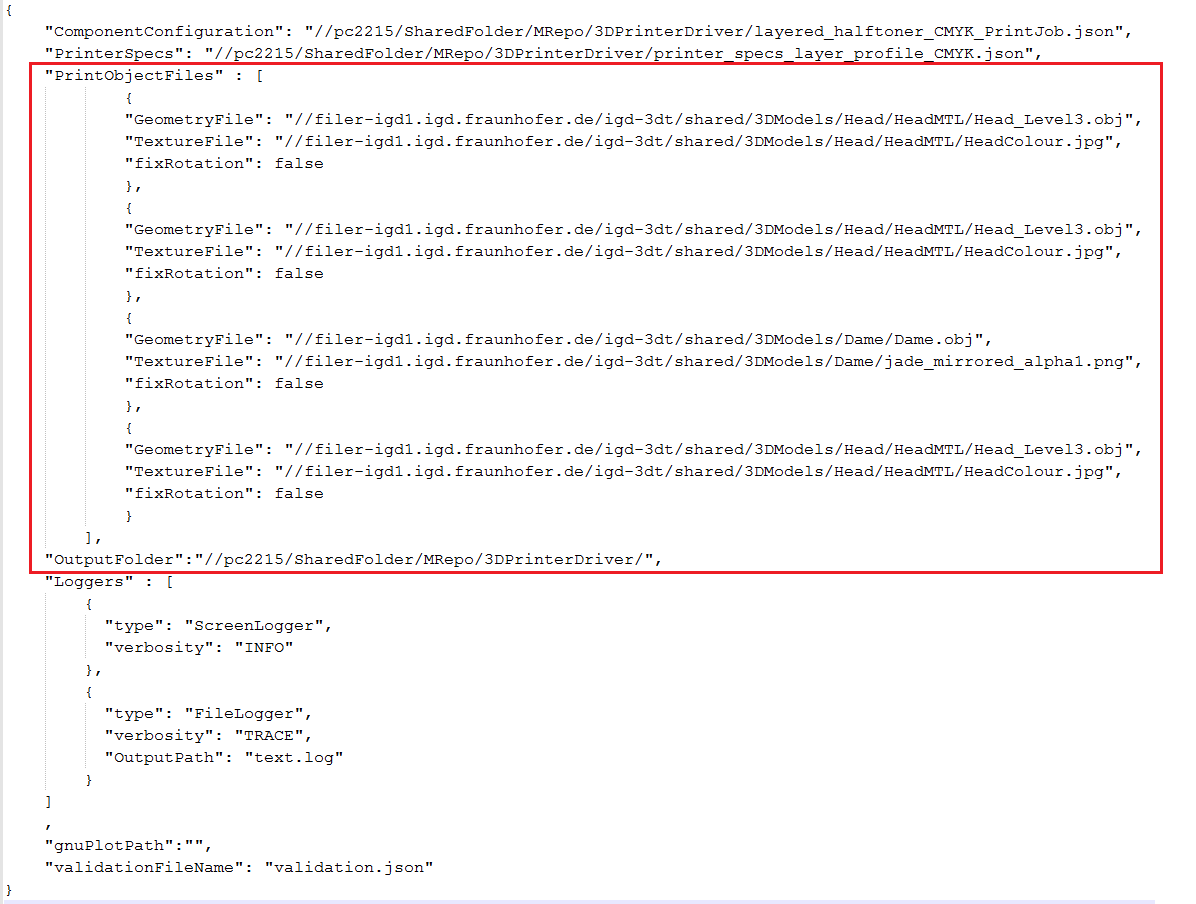
\includegraphics[scale=0.6]{MasterConfigurationFile.png}
\caption{Master Configuration file}
\label{fig:MasterConfigurationFile}
\end{figure}

\begin{figure}[ht!]
\centering
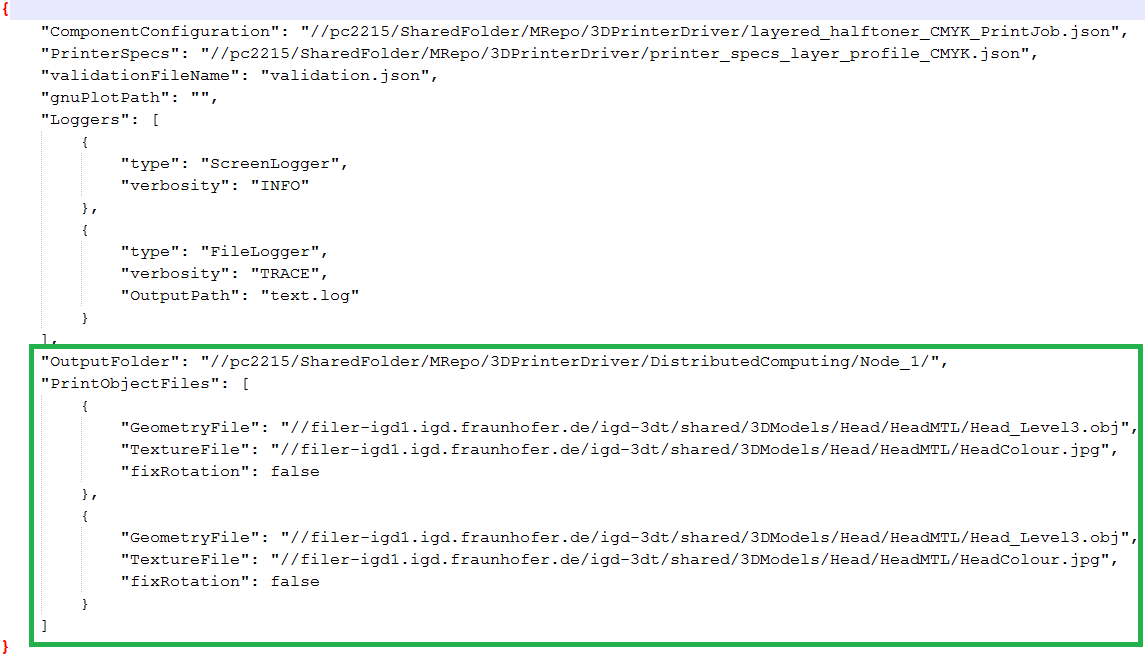
\includegraphics[scale=0.6]{Slave1ConfigurationFile.png}
\caption{Slave 1 Configuration file}
\label{fig:Slave1ConfigurationFile}
\end{figure}

\begin{figure}[ht!]
\centering
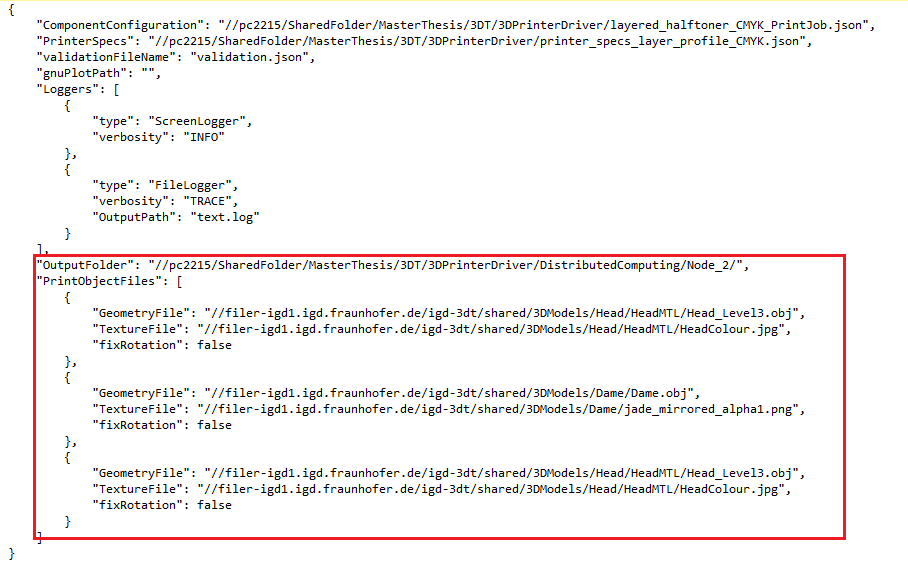
\includegraphics[scale=0.6]{Slave2ConfigurationFile.png}
\caption{Slave 2 Configuration file}
\label{fig:Slave2ConfigurationFile}
\end{figure}

This prototype is possible only if the cluster nodes have read/write permission to the shared network file system where the geometry, texture files and input/output folders are stored /created. The \textit{MasterDistributor} creates a unique path for each slave using the rank of the slave and writes the configuration file to this path. It then communicates to the slave only the path where the slave can find the configuration file. The sequence diagram in the Figure \ref{fig:SequenceDiagram1} summarizes the communication between the master and the slaves.  

\begin{figure}[ht!]
\centering
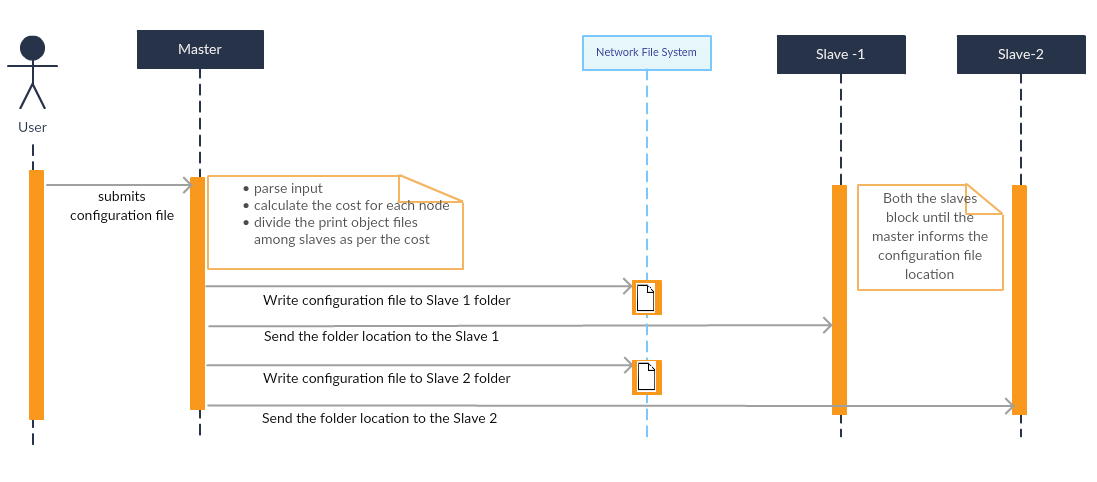
\includegraphics[scale=0.6]{SequenceDiagram1.png}
\caption{Master-slave input communication}
\label{fig:SequenceDiagram1}
\end{figure}

The advantages of distributing the sub-tasks through the configuration file are:
\begin{itemize}
\item \textbf{Design simplicity}: The most important aspect of this design is it's simplicity as the \textit{SlavePrintingSoftware} pipeline does not need to be modified greatly with respect to the serial 3D Printing pipeline, which means that it is almost similar to running a single instance of the non-distributed version of the 3D Printing pipeline. 
\item \textbf{Lower Communication Overhead}: Slave nodes are blocked until the master communicates the configuration file path to each slave. Communication of the file path is faster as it is less number of bytes to be exchanged among the nodes as compared to the number of bytes to be sent when print jobs are distributed .
\item \textbf{Faster Disk I/O}: The configuration file read and writes i.e. disk I/O (both at the master and slave) are much faster than sending the print job as series of bytes because of the additional steps (refer to section detailing the second prototype) that need to be performed while sending the print jobs. It is simpler implementation as communicating the print jobs as series of bytes would require serialization and deserialization of the print jobs with an additional effort of communicating the size along with texture information for each print object.
\item \textbf{No serialization and deserialization}: As the configuration files are in JSON format, there are very efficient library functions which allow to read and write the files with ease. As the format of the files is quite standard, there is no need for serialization and deserialization of the files even if the nodes have varying underlying system architecture.        
\end{itemize}

The disadvantages of distributing the sub-tasks via configuration file are: 
\begin{itemize}
\item \textbf{Dependency on shared network file system}: This prototype has a strong requirement that the nodes have a shared network file system and each node must have read access to the model texture/geometry file along with write access to the output folder to dump the partial output. If the print jobs are communicated as stream of bytes, it is possible to get rid of this requirement.
\item \textbf{Performance overhead}: The configuration file, model geometry and texture files are parsed twice, once by the master to create the prints jobs needed for cost computation and once by the slaves for actual computation. This leads to redundant execution of the \textit{FileParserPj} and \textit{PrintJobOrganizer} at both master and slave nodes which accumulates to a significant performance overhead (refer to the Section).
\item \textbf{Performance bottleneck at the master}: As the files are read and written to the shared network file system, the network bandwidth limits the speed of the disk I/O. With increase in number of slave nodes, the load at the master to write the configuration file per slave increases which may become a performance bottleneck. 
\end{itemize}

\subsubsection{Sub-Task Distribution}

The sub-tasks are distributed by the \textit{MasterDistributor} component based on a cost function. The goal of the distribution is to allocate equal work to each slave i.e. none of the slaves are over-worked and all of them finish the work almost at the same time. One of the main reasons which makes it important to achieve load balancing is to ensure better utilization of the cluster resources, a cluster as a whole will perform well only if each of the nodes do equal work leading to none of the nodes being the bottleneck. 

The cost function used for distribution of the tasks evaluates the cost of each work item and allocation of work item among the slave nodes is done such a way that total cost of allocated work items is equal for each node. The cost for each work item may vary depending on the work item, for example for print objects, the size or the print volume of the print objects could be seen as cost of the work item, or priority assigned to the print objects can be another way to evaluate the cost. 
\newline

\subsubsection{Naive cost function implementation }\label{costFunc}
Each print object \textit{\begin{math}O_{i}\end{math}} has an axis-aligned bounding box \textit{\begin{math} B(O_{i}) \end{math}}. The minimum bounding box-\textit{min(B(\begin{math}O_{i}\end{math}))} and maximum bounding box-\textit{max(B(\begin{math}O_{i}\end{math}))} is calculated. Using \textit{min(B(\begin{math}O_{i}\end{math}))} and \textit{max(B(\begin{math}O_{i}\end{math}))}, the width(\textit{W}), height(\textit{H}), and length(\textit{L}) of each print object is calculated as per equation \ref{eq:length}

\begin{equation}
\label{eq:length}
\begin{aligned}
W= max(B(O_{i})).y-min(B(O_{i})).y \\
H= max(B(O_{i})).z-min(B(O_{i})).z \\
L= max(B(O_{i})).x-min(B(O_{i})).x \\
\end{aligned}
\end{equation}

The volume (\begin{math}V^i\end{math}) of the bounding box \begin{math}B(O_{i})\end{math} is calculated using the equation \ref{eq:volume}.

\begin{equation}
\label{eq:volume}
V^i= WHL
\end{equation}

The total sum of the volumes of \textit{k} print objects calculated using equation \ref{eq:Sum} 

\begin{equation}
\label{eq:Sum}
\begin{math} V_{Total} \end{math} =\sum\limits_{i=1}^{k}{V^i}
\end{equation}

Threshold (for each node in a cluster of size \textit{n-1}) calculated using equation \ref{eq:threshold} is used for allocating the sub-tasks to the slaves. The cluster size considered is \textit{n-1} as the master is not allocated any sub-task and is hence excluded from the cluster of slaves.

\begin{equation}
\label{eq:threshold}
T =\frac{1}{n-1}\sum\limits_{i=1}^{k}{V^i}
\end{equation}

The allocation of the sub-tasks is done using the greedy approach. The list of volumes calculated using equation \ref{eq:volume} is sorted in the  descending order. Then the allocation of the object is done in a round-robin fashion to each slave  until the allocated total volume  for the node is greater than or equal to the threshold. If the threshold is already reached for the node, then the node is skipped. The allocation of the print object stops when each node\textquotesingle s capacity has been consumed or all the print objects are assigned. The listing \ref{lst:ppga} summarizes the distribution logic.

\begin{lstlisting}[language=C++,label={lst:ppga},caption={Distribute Tasks- Greedy Approach}]
DistributeTasks(VolList,threshold,NumNodes)
{
	std::sort(VolList.begin(), VolList.end(),std::greater<>()); // sort in descending order
	int listOfSum(NumNodes-1)={0};
	int vlSize= VolList.size();
	int nodeInd= 1;
	int allocatedIndexList(NumNodes-1);
	for (size_t ind = 0; ind < vlSize;)
	{
			if (listOfSum[nodeInd] < threshold)
			{
				sumList[nodeInd] = sumList[nodeInd] + tempList[ind];
				indList[nodeInd].push_back(ind);
				ind++;
			}
			
			if (nodeInd == NumNodes-1)
				nodeInd = 0;
			else 
				nodeInd++;
	}
}
\end{lstlisting}

\subsection{Slave Partial Output} \label{SRepoComp}

The \textit{SlaveReporter} component receives the container of \textit{slices} whose size is equal to the \textit{chunk} size, as input from the previous component in the pipeline. At each of the slaves, the container actually contains the partial \textit{slices} which are sent to the master for merging.  Each slice internally stores the width, height and the buffer which contains the material id of the assigned material at varying \textit{(x,y)} coordinate. As the cluster may contain heterogeneous machines with varying system architecture, to ensure proper interpretation of the slices at the master, the slices are serialized. \textit{Serialization} of the slices includes serializing the width, height (unsigned integers to same size), buffer to an output stream (std::ostream). The behavior of the \textit{SlaveReporter} component is summarized in the Figure \ref{fig:SlaveReporterActivityDiagram}. \newline
\begin{figure}[ht!]
\centering
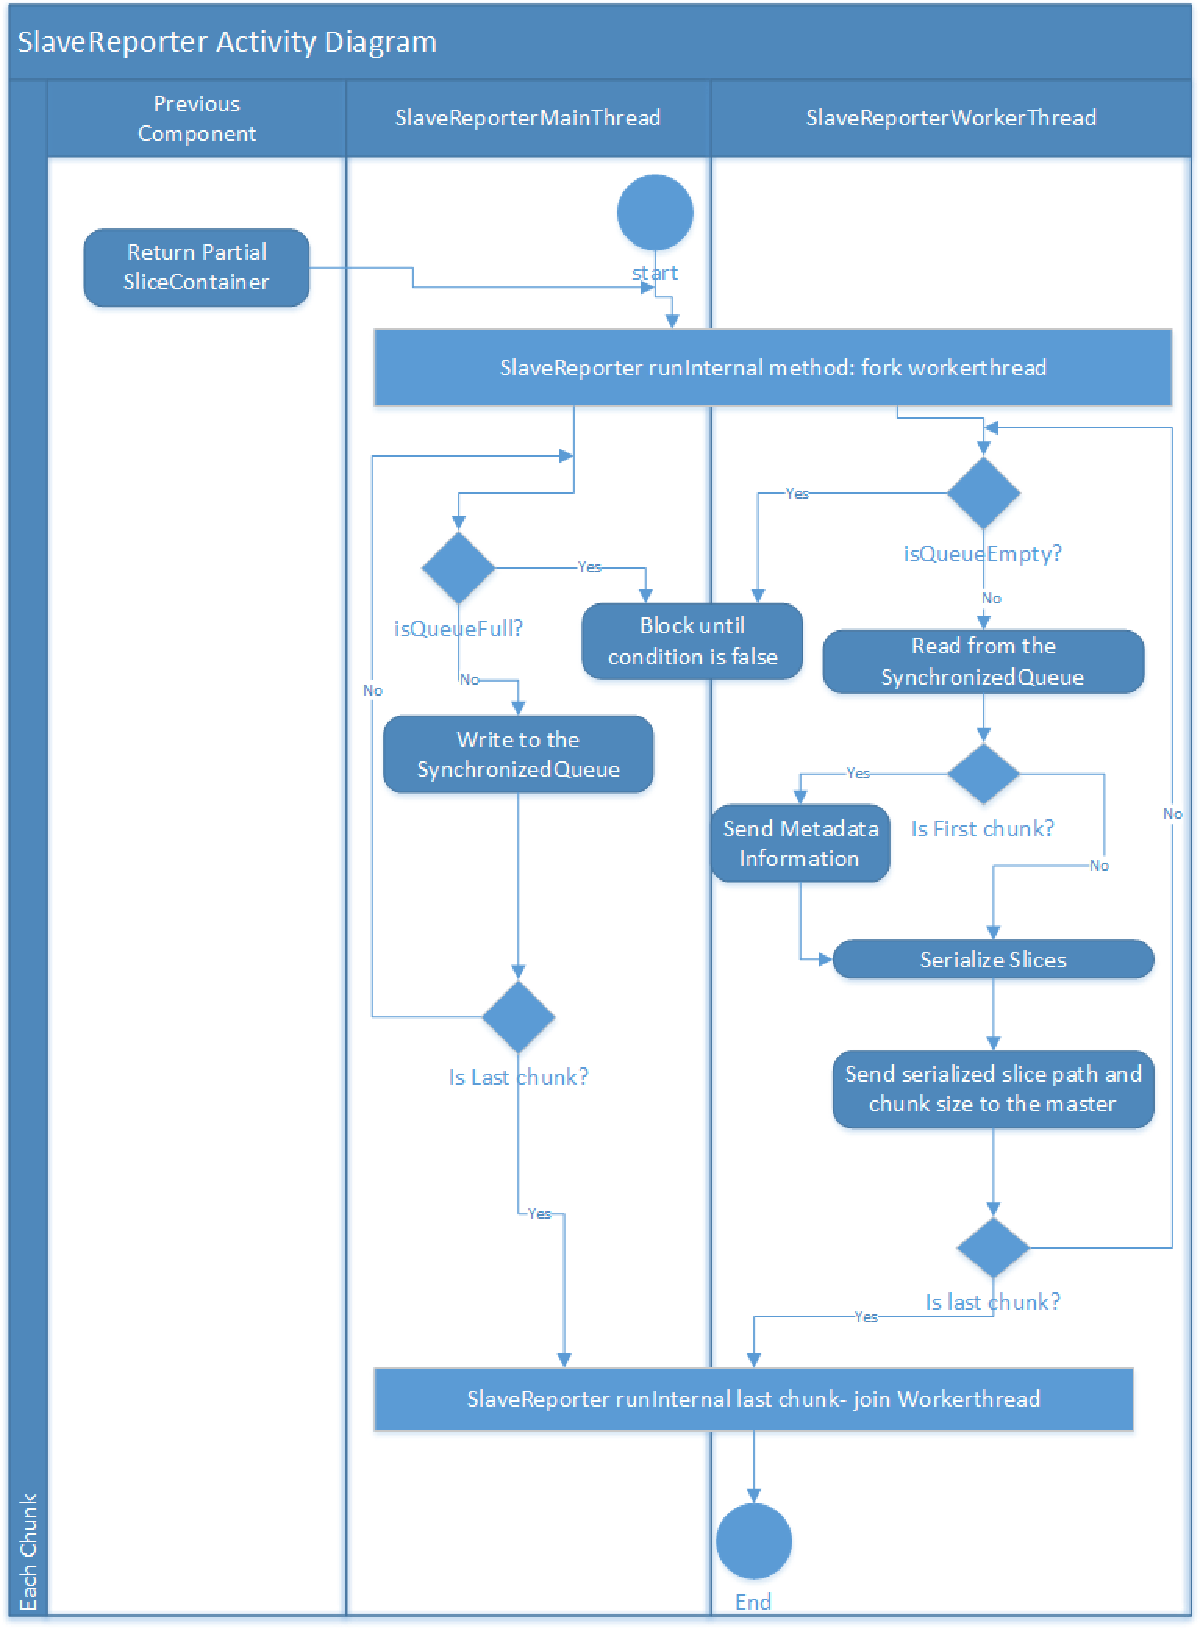
\includegraphics[scale=0.8]{SlaveReporterActivityDiagram.PNG}
\caption{\textit{SlaveReporter} Activity Diagram}
\label{fig:SlaveReporterActivityDiagram}
\end{figure}

\textbf{Analysis of component behavior}
\newline
The \textit{SlaveReporter} component is multi-threaded and uses a synchronized queue for inter-thread communication. The \textit{runInternal} method of each component is the main thread of execution i.e. the cuttlefish process, whereas in the first run of this method a worker thread is created which executes asynchronously to perform certain tasks. The main thread interacts with the next and previous components of \textit{SlavePrintingSoftware} whereas the worker thread interacts with the main thread and worker threads of \textit{MasterPrintingSoftware-MasterMerger} component. \newline

The interaction between the main thread and the worker thread can be viewed as the classic producer consumer problem, see Figure \ref{fig:ProducerConsumerProblem}, where in the main thread produces the partial slices which are consumed by the worker thread and serialized. Each chunk of partial slices is one work item produced by the main thread and inserted in the buffer. Depending on the type of buffer, there might be varying number of synchronization points between the threads. In the current design, the buffer is implemented as a queue of limited size i.e. a bounded buffer. As the buffer is of fixed size, there are two conditions which lead to blocking either the main thread or the worker thread. As the main thread acts as the producer, it blocks when the buffer is full (i.e. slow consumer) and waits on a condition indicating at least one free slot in the buffer. The worker thread acts as the consumer and blocks when there is no work item to consume and waits until there is at least one full slot. \newline

\begin{figure}[t]
\centering
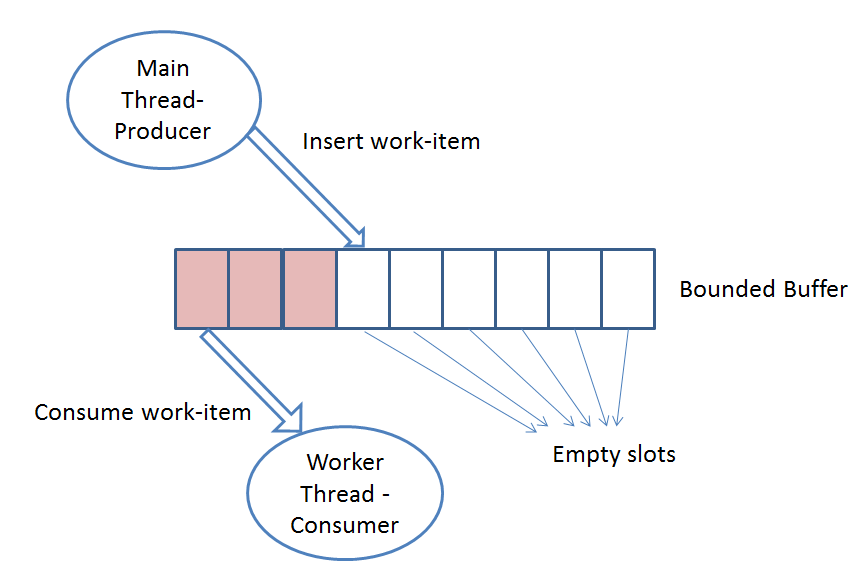
\includegraphics[scale=0.6]{ProducerConsumerProblem.PNG}
\caption{Producer-Consumer Problem}
\label{fig:ProducerConsumerProblem}
\end{figure}

The worker thread performs the task of serialization and once each chunk of slices is serialized, it communicates with worker thread of \textit{MasterPrintingSoftware-MasterMerger} component the chunk size- it acts as a way of synchronization of the worker threads between the components. The worker thread sends some meta-data  only for the first chunk of slices which includes slice height, slice width, chunk size, total number of slices. This meta-data is used by the main thread of \textit{MasterPrintingSoftware-MasterMerger} component for creating full slices.\newline

The advantages of \textit{SlaveReporter} component design are:
\begin{itemize}
\item \textbf{Separation of concerns}: The main thread is responsible for assigning the work to the worker thread and returns to continue with execution of the pipeline with the next chunk whereas the worker thread is responsible for communication and serialization.  
\item \textbf{Asynchronous communication}: The worker thread performs the blocking calls for synchronization with worker threads of \textit{MasterPrintingSoftware-MasterMerger} component. As it does so asynchronously with respect to the main thread, the communication will never lead to blocking the main thread. Both the main thread and worker thread execute in parallel.
\end{itemize} 

The disadvantages of \textit{SlaveReporter} component design are:
\begin{itemize}
\item \textbf{Synchronization Overhead}: The main thread and the worker thread need to synchronize access to the shared buffer so as to avoid race condition along with blocking calls on buffer full/ empty condition. The size of the buffer influences the performance of the solution i.e. if unlimited buffer is used the producer will never block whereas if no buffer is used there is no need for explicit synchronization as producer produces only one item and the consumer consumes it after it is produced.
\item \textbf{Increased implementation complexity}: Synchronization between the threads leads to added implementation complexity and if not managed properly might lead to deadlock. 
\end{itemize} 

\subsection{Partial Output Merging at Master} \label{MMComp}

The partial slices serialized by the slaves are de-serialized at the \textit{MasterMerger} component. The \textit{MasterMerger} component creates a worker thread per slave node in the cluster which interacts with the worker thread created by the \textit{SlaveReporter} component. The main thread of the \textit{MasterMerger} component synchronizes with worker threads at various points during the execution. The worker threads of \textit{MasterMerger} component first wait to receive the meta-data information from the \textit{SlaveReporter} component worker thread. After they have received the slice height, width, total number of slices and chunk size, they synchronize with the main thread and indicate the receipt of the meta-data. The worker threads then wait to receive the chunk size of the serialized data from the worker threads of \textit{SlaveReporter} component, the receipt of the chunk size is the indication that slices are serialized and ready for deserialization. On receiving the chunk size, they start with deserialization of the slices and create a container of deserialized partial slices. \newline

In the meantime, the main thread uses the received meta-data information from the slaves and then creates the container of the full slices. The worker threads at the master node continue to deserialize the chunk they received from the slaves and block until the container of full slices is created by the main thread and ready to be written. On signaling of availability of the container by the main thread, the worker thread then proceed with writing the partial slices to the full slices.\newline 

Each worker thread has a dedicated section in the full slice where it writes to, which helps to avoid write conflicts on the shared storage. The main thread waits until all the worker threads have finished writing the partial slices to the full slices and has container of full slices ready. The main thread then continues to proceed with the pipeline with fully merged slices whereas worker threads continue to deserialize the slices or communicate with worker threads of the slave or write the partial slices to the full slice in the container provided by the main thread. The activity diagram in the Figure \ref{fig:MasterMergerComponent} shows the activity of the main thread and worker threads of \textit{MasterMerger} component. \newline
   
The main thread at the master computes the full slice height (\begin{math}H_{\textit{f}}\end{math}), full slice width (\begin{math}W_{\textit{f}}\end{math}), offset (\begin{math}Of_{\textit{i}}\end{math}) for each worker thread (\begin{math}W_{\textit{i}}\end{math}), and total number of full slices (\begin{math}N_{\textit{f}}\end{math}). The full slice height \begin{math}H_{\textit{f}}\end{math} is computed as the addition of all the partial slice heights. If the full slice height \begin{math}H_{\textit{f}}\end{math} is exceeding the print bed height, then full slice height \begin{math}H_{\textit{f}}\end{math} is set to the print bed height- \textit{max(H)}. The height is calculated as the addition of partial slice heights because the partial slices from the slaves are written one below the other in y-axis until either the print bed height is reached or each of the slave node partial slices are placed. If the print bed height \textit{max(H)} is reached and there are still pending slave partial slices to be fit in the full slice, then the maximum partial slice width is taken as the x-offset and the remaining slices are then places along the y-axis again with each having the x-offset. The listing \ref{lst:fsh} summarizes the logic of full slice height calculation. \newline

\begin{lstlisting}[language=C++,label={lst:fsh},caption={Calculate full slice height}]
int fullsliceHt(std::vector<int> listOfpartilSliceHt)
{
	int maxAllowedHt = getPrintBedHeight(); // get the print bed height
	int totalht(0);
	for(size_t i =0;i<listOfpartilSliceHt.size(),i++)
	{
		totalht =  listOfpartilSliceHt[i] + totalHt;
	}
	if(totalht > maxAllowedHt)
	{
		totalHt= maxAllowedHt; 
		m_xOffsetNeed=true; // to indicate that x-offset will be added to some slaves
	}
	return 	totalHt;
}

\end{lstlisting}

The full slice width (\begin{math}W_{\textit{f}}\end{math}) is calculated as the maximum of the all the partial slice widths. If the total height calculated exceeds the print bed height, then total slice width is calculated as the sum of all slice widths. If the total slice width exceeds the print bed width- \textit{max(W)}, then there is no way to fit all the partial slices in the given print bed and hence some of the slaves need to be dropped. If the total slice width (\begin{math}W_{\textit{f}}\end{math}) does not exceed the print bed width \textit{max(W)}, the full slice width (\begin{math}W_{\textit{f}}\end{math}) is equal to the sum of individual partial slice widths. The full slice width calculation is summarized in the listing \ref{lst:fsw}.\newline     


\begin{lstlisting}[language=C++,label={lst:fsw},caption={Calculate full slice width}]
int fullsliceWd(std::vector<int> listOfpartilSliceWd)
{
	int maxAllowedWd = getPrintBedWidth(); // get the print bed width
	int totalWd(0);
	if(m_xOffsetNeed) // this is set to true if the total sum of slice heights > print bed height.
	{
		for(size_t i =0;i < listOfpartilSliceWd.size(),i++)
		{
			totalWd =  listOfpartilSliceWd[i] + totalWd;
		}
		if(totalWd > maxAllowedWd)
		{
			m_DropSlaves=true; // to indicate that some slaves need to be dropped
		}
	}
	else
	{
		for(size_t i =0;i < listOfpartilSliceWd.size(),i++)
		{
			totalWd = totalWd > listOfpartilSliceWd[i]? totalWd : listOfpartilSliceWd[i];
		}
	}
	return 	totalWd;
}
\end{lstlisting}

The total number of full slices is the maximum value from the received total number of slices from the slaves. The main thread needs to keep track of the individual total number of slices from each slave node so as to ensure that the master does not block for a worker thread to write to the full slices when there are no more partial slices left. 

\begin{figure}[ht!]
\centering
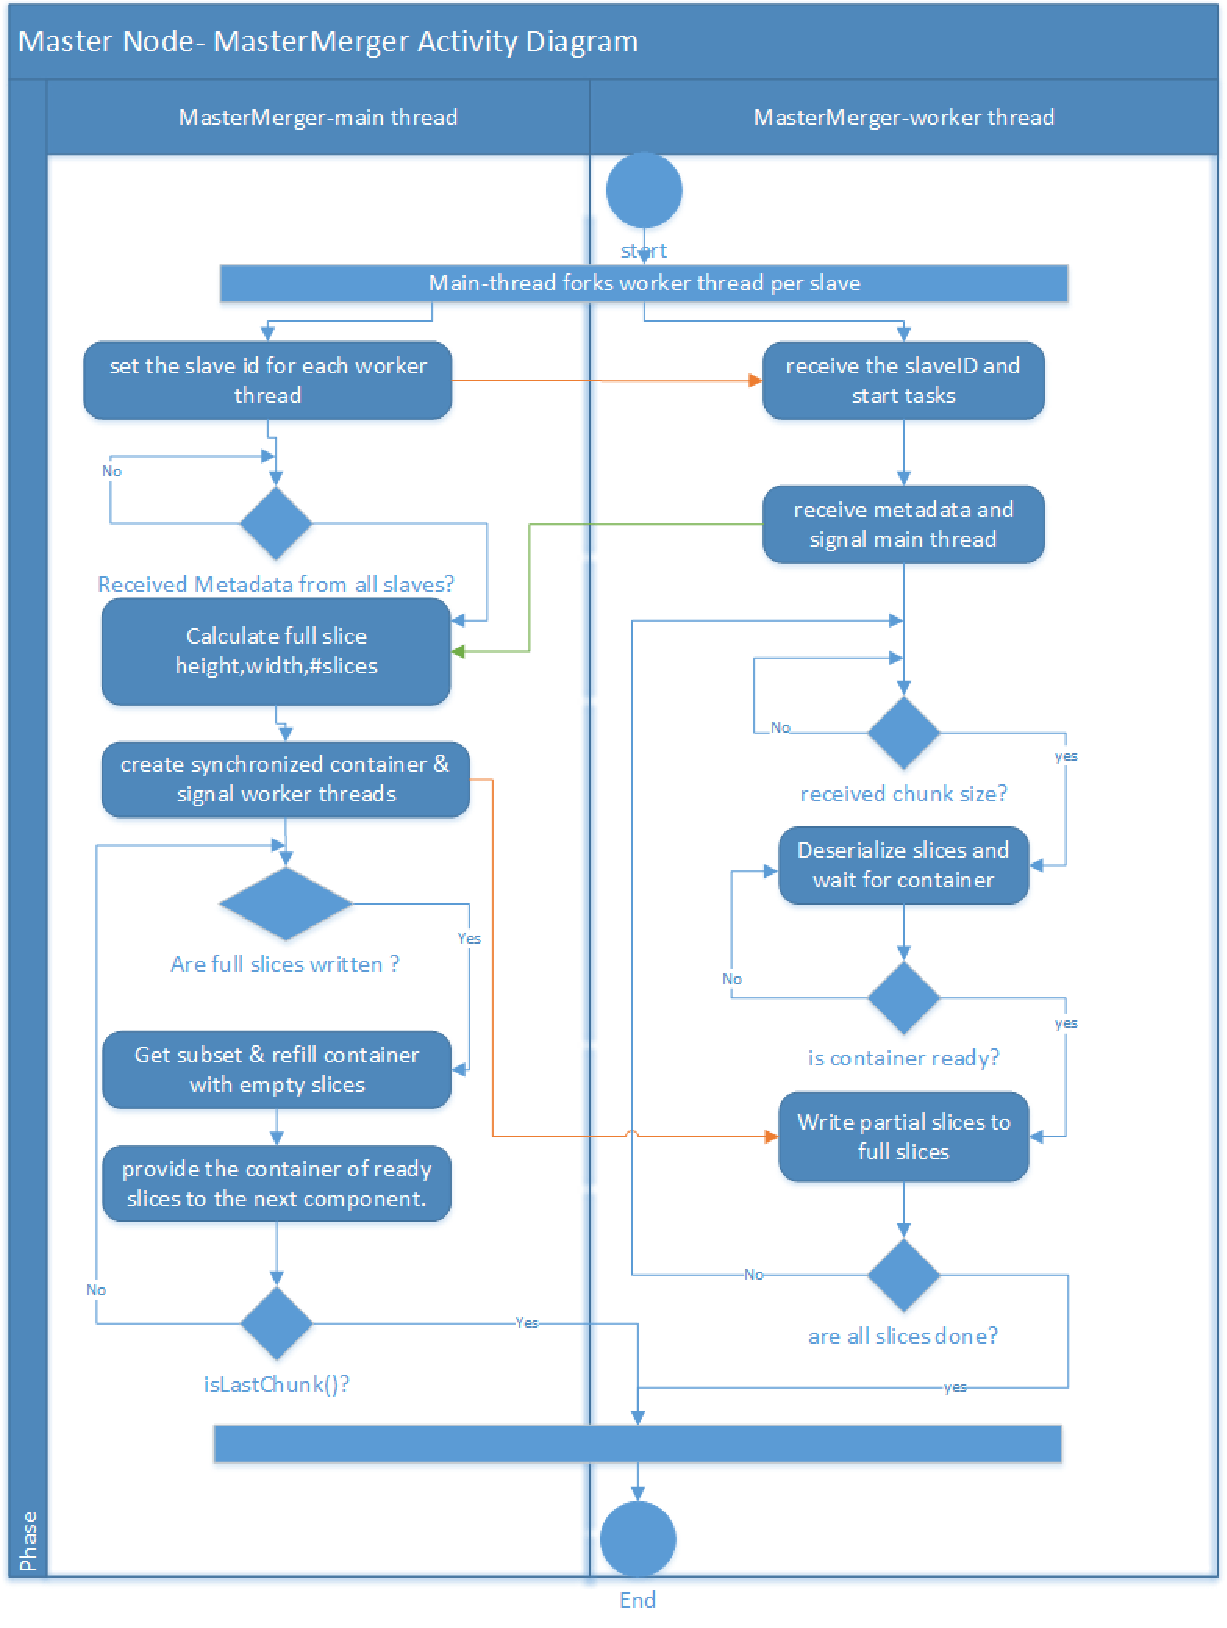
\includegraphics[scale=0.85]{MasterMergerComponent.PNG}
\caption{\textit{MasterMerger} Component- Activity Diagram}
\label{fig:MasterMergerComponent}
\end{figure}

The slice container to be provided by the main thread is a synchronized slice container which means that while removing the individual slices or subset of slices or adding the slices to the container, each thread needs to obtain the lock over the container and modify the container thereafter. The use of synchronized container ensures no data race on the shared data structure. \newline 

The advantages of the \textit{MasterMerger} component design are:  
\begin{itemize}
\item \textbf{Separation of concern}: A worker threads for each slave node helps to maintain the separation of the responsibilities among the worker threads as each worker thread is responsible for the assigned slave node.
\item \textbf{Asynchronous communication and exploiting the possible parallelism}: The worker threads for each slave node communicate with the worker thread of the \textit{SlaveReporter} component asynchronously without blocking the execution of the main thread.The worker threads perform deserialization of partial slaves and write to their assigned section in the full slices simultaneously without write conflicts amongst them. The main thread also continues to work on computing the full slice height, width etc while the worker threads are deserializing and when the worker threads are done writing to the full slice container, return the full slice container to proceed with next  component execution in the pipeline in a chunk-wise fashion. This design maintains the streaming architecture of the original non-distributed version of the pipeline. 
\end{itemize}

The disadvantages of the \textit{MasterMerger} component design are:
\begin{itemize}
\item \textbf{Synchronization Overhead}: As there are many synchronization points during the execution where either the worker threads block or the main thread block, it might lead to overhead in the execution run time. Also the synchronization leads to added code complexity. 
\item \textbf{Limited possibilities of partial slice arrangement}: As the arrangement of the partial slices in the full slices is done, there is a possibility of not achieving the optimal arrangement leading to the waste of the print area along with incapability of accommodating each slave. This might lead to dropping one or more slaves from the merging process to enable making the best possible use of the work done by the slaves.  
\item \textbf{Possibility of deadlock}: The main thread at the master blocks until each slave has received the meta-data or written to the full slices. The main thread might remain blocked if one of the slaves crashes which will eventually lead to a deadlock as other slaves might get blocked until the main thread refills the container with new empty slices. To avoid this, use of timeouts could be done. If the worker thread for a particular slave does not respond within the timeout period, then slave could be dropped. The timeouts shouldn't be too small leading unnecessary dropping of the slaves or too long leading to increased execution time overhead even when the blocking slave has crashed. The use of timeouts adds further code complexity.
\end{itemize}

\section{Prototype II- Input/Output independent of Network File System }

As discussed in the Section \ref{protoI}, the prototype I functions only if there is a shared network file system amongst the cluster nodes. The network file system is primarily used to communicate between the nodes the work load (i.e. the configuration file) and the partial output. So, to get rid of this dependency the communication between nodes must be done by sending the data through the network as a stream of bytes and not via disk I/O. The prototype II involves two major changes as compared to Prototype I: 
\begin{itemize}
\item Independence from Network File System 
\item Format of the work item allocated to the slaves
\end{itemize}  

The architecture of the distributed cuttlefish pipeline remains almost the same with two minor changes, the \textit{MasterDistributor} component is replaced by another component called as \textit{MasterPJDistributor} in the \textit{MasterPrintingSoftware}, and in the \textit{SlavePrintingSoftware}, the component \textit{SlavePJCollector} replaces the components \textit{FileParserPJ} and \textit{PrintJobOrganizer}. These changes in the printing software are explained in the following subsections. 

\subsection{Selection of the prototype}

The algorithm for performing the distributed computing progresses in the same fashion as described in the Figure \ref{lst:FC}. The configuration file submitted as input by the user to the cuttlefish application consists of a tag called as \textit{DistributionPrototype} whose value indicates the distribution prototype to be used. The valid values for this tag are 1 for prototype I and 2 for prototype II. The master node parses the configuration file and depending on the value of the \textit{DistributionPrototype} tag, it creates the components of \textit{MasterPrintingSoftware} and sends the prototype value to the slave nodes. The slave nodes wait to receive the prototype value and then add the components of \textit{SlavePrintingSoftware} depending on the received value. \newline

\subsection{Selection of Printing Software Components}
In the prototype I, the slave nodes receive the path where they could find the configuration file containing the information about of the assigned print models, texture information, component configuration for the printing pipeline and the printer specification. Just sending the prototype value is not sufficient for the slave nodes to create the \textit{SlavePrintingSoftware}. The master needs to send to each slave node all the information which was earlier contained in the main configuration file along with the information from the other files included in the main configuration file. So master should send the JSON data describing the component configuration and printer specification. Each slave node after receiving the prototype value decides what is the next information that it should wait for from the master node. For prototype I, the slave nodes wait for the main configuration file path and for prototype II, they wait for the component configuration and the printer specification description. The component configuration description depends on the user's choice of components and the configuration of each component. As the description may vary, the master first sends the size of the data followed by the data describing the component configuration. Similar to the component configuration, the printer specification description depends on the printer settings provided by the user via the printer specification file. As description of the printer specification is subject to vary depending on the available 3D printer, size of the data is sent to the slave nodes followed by the data describing the printer specification.\newline 

\subsection{Distribution of the work load to the slave nodes}

After communicating the information related to the prototype, component configuration and printer specification, the next step for the master node is to create the work load for each slave. The \textit{MasterPrintingSoftware} starts with the steps similar to prototype I i.e. parse the configuration file provided by the user and create the print job. The components responsible for doing these tasks namely, \textit{FileParserPJ} and \textit{PrintJobOrganizer}, remain unchanged. The print job is then passed to the \textit{MasterPJDistributor} component. From this point onwards the behavior of the pipeline varies for prototype II. The \textit{MasterPJDistributor} component is responsible for distributing the print jobs to the slave nodes instead of writing the configuration files per slave node. The cost function used to distribute the load amongst the nodes is the same as prototype I. The difference is the format in which the work load is assigned to the slave nodes. For each slave, a new print job containing the print objects (distributed as per the cost function) is created. Each newly created print job is a set of the print objects such that, the sum of the volumes of the print object bounding boxes is less than or equal to the threshold calculated using the cost function. The goal of the cost function is to have equal work load for each slave node so that each one of them finishes the chunk-wise computation almost at the same time.\newline

The steps performed by \textit{MasterPJDistributor} component are as follows: 
\begin{enumerate}
\item The \textit{PrintJobOrganizer} creates the print job and passes the print job to the \textit{MasterPJDistributor} component. 
\item In the \textit{MasterPJDistributor} component, the cost function is calculated using the print object bounding boxes. The calculation of the cost function is same as described in the subsection \ref{costFunc}.
\item Using the threshold calculated in the step 2, the distribution of the print objects is done such that sum of the volumes of the print object bounding boxes (assigned to each slave) is less than or equal to the threshold.
\item The set of print objects assigned to each slave is then packed into a print job per slave. 
\item The print job is then serialized to a stream of bytes and sent to the slaves. As the size of the print job may vary, the size of the serialized print job is sent to the respective slave first followed by the print job data. 
\item Each print object has texture information which is used to generate the desired appearance. The texture data is stored in the master node GPU memory when the print job is created. For the slave nodes to perform the computation and generate the partial slices correctly, the slave nodes need the texture information which should be sent by the master. The texture data size may also vary per print object and hence, the size of serialized texture data is sent first followed by the serialized texture data.   
\end{enumerate}

So to summarize the information sent by the master node to each slave node:
\begin{itemize}
\item prototype value indicating the chosen distribution type
\item size of the component configuration description 
\item component configuration description
\item size of the printer specification description 
\item printer specification description
\item size of the serialized print job 
\item serialized print job 
\item for each print object in the print job, size of texture data and texture data  
\end{itemize}

\subsection{Work Load Collection and Computation}

At the slave nodes, the first step performed is receiving the type of distribution i.e. the prototype value set by the user via the configuration file submitted to the master node. After it receives the prototype value, the slave node decides which is the next information it should wait for. For prototype II, the slave nodes wait for the component configuration. Each slave node in the cluster receives the same component configuration from the master. As the component configuration is set by the user and the size of the JSON string describing the component configuration may vary in size, the slave nodes first receive the size of the string and allocate the buffer of the appropriate size to receive the actual component configuration string. Followed by the component configuration, the slave nodes waits to receive the printer specification, similar to component configuration information, first the size of the JSON string holding the printer specification followed by the actual string. \newline   

The slave nodes then proceed to create the printing software containing the needed components. Similar to the prototype I, the \textit{SlavePrintingSoftware} does not contain any output component. As the work load received by the slaves nodes in the prototype II is a print job, The components \textit{FileParserPJ} and \textit{PrintJobOrganizer} are not included in the \textit{SlavePrintingSoftware}, instead a new component called as the \textit{SlavePJCollector} is included. The \textit{SlavePJCollector} component receives the size of the serialized print job sent by the master and allocated the buffer to receive the actual serialized print job as stream of bytes. It then deserializes the received data to create the print job. For each print object contained in the print job, it waits to receive the texture information. The slaves receive the size of the texture data, allocate the buffer for the texture data and then receive the texture data. The received texture data is then deserialized and saved in the memory of the node. The rest of pipeline remains unchanged until the \textit{SlaveReporter} component.\newline

The \textit{SlaveReporter} component, similar to the prototype I, receives the partial slices and reports them to the master node. As the nodes within the cluster do no have a shared network file system, the slices which are reported to the master node are in form of stream of bytes instead of files written to the disk. The value of the selected distribution type is set at the time \textit{SlavePrintingSoftware} creation as \textit{persistent} data- it is a piece of information accessible by all the components of the pipeline. \textit{SlaveReporter} fetches the prototype value from the persistent storage before it proceeds with rest of the computation. \newline

The \textit{SlaveReporter} component sends the meta-data information which is the partial slice height, width, total number of slices for the assigned work load and first chunk size. For the prototype II, it skips sending the path where the master node would find the partial slice file. For each chunk of partial slices to be sent to the master, the slave begins by informing the size of the chunk followed by serialization of the slices. Through serialization of the slices it converts the slices to stream of bytes. The size of the serialized slice is sent to the master which allows the master to allocate the buffer of appropriate size and then send the serialized slice data. The \textit{SlaveReporter} component design remains unchanged and is as described in the subsection \ref{SRepoComp}.

\subsection{Creation of the full slices}

At the master node, after assigning the work load to the slave nodes, the \textit{MasterMerger} component is executed. It is in charge of collecting the partial slices from the slave nodes and merging them to form full slices. The \textit{MasterMerger} component, similar to the \textit{SlaveReporter} component, fetches the prototype value from the persistent storage which is saved when the instance of the \textit{MasterPrintingSoftware} is created. There is no huge difference in how the component performs the merging of the partial slices but rather how it receives the partial slices from the slave nodes. The component design remains unchanged and is as described in the subsection \ref{MMComp}. Each worker thread begins by receiving the meta-data information from their respective slave node. For the prototype II, the worker thread does not receive the path where the partial slices files are written by the slave. After receiving the chunk size, the worker threads receive the size of the stream of bytes slice-wise, allocate the buffer and receive the stream of bytes. They then deserialize the stream of bytes to partial slice and store them in the partial slice container. The rest of the steps until the merging of partial slices to full slice and passing them to the output component remains unchanged.

The information communicated between the master and slave nodes is summarized in the Figure \ref{fig:ProtoII}.

\begin{figure}[!t]
\centering
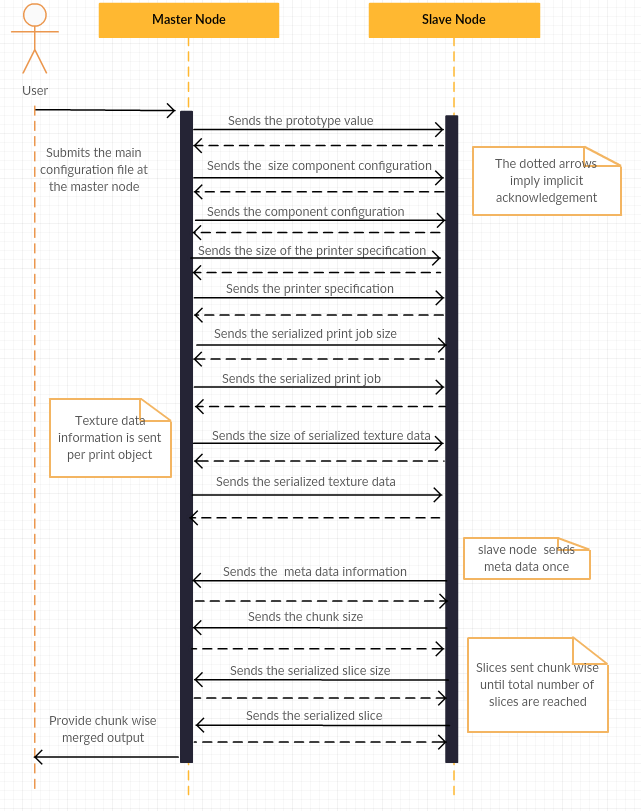
\includegraphics[scale=0.85]{ProtoII_SequenceDiagram.PNG}
\caption{Communication between slave and master nodes}
\label{fig:ProtoII}
\end{figure}


\section{Serialization and Deserialization of Data}

The nodes forming the cluster used for distributed computing may not always be homogenous, which means that each node may be different in terms of the system architecture, computation capacity and memory. Due to such heterogeneity, the representation of the user defined data types (i.e. in our case objects) may vary as the "endianness" of the nodes might differ \cite{ObSerDeser}. To ensure that each node interprets the data correctly, the objects are "flattened" to stream of bytes or a string before sending it the destination, also known as serialization of the objects. At the destination node, the received stream of bytes are "unflattened" to reconstruct the objects, which is known as deserialization \cite{yadav2016system}. The Figure \ref{fig:SerDeser} summarizes the serialization and deserialization process used in cluster computing.

\begin{figure}[!t]
\centering
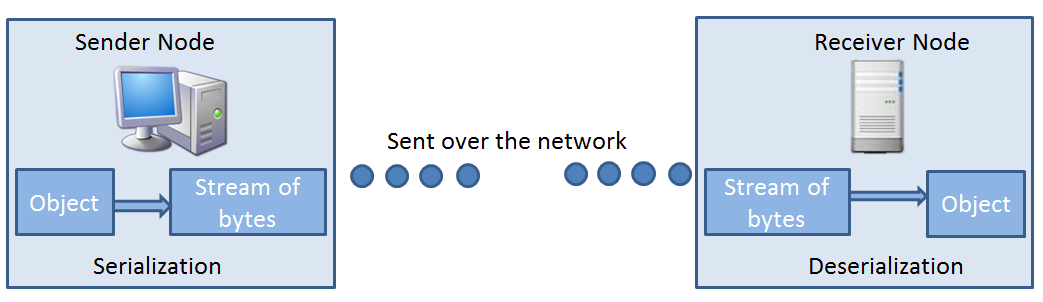
\includegraphics[scale=0.65]{SerDeser.PNG}
\caption{Serialization and Deserialization}
\label{fig:SerDeser}
\end{figure}
  